%%% ------------ 1. CORE & LAYOUT ------------ %%%
\documentclass[11pt]{article}
\usepackage[english]{babel}
\usepackage[letterpaper, margin=1in]{geometry}
\usepackage{authblk}      % Author affiliations
\usepackage{setspace}     % Linespacing
\usepackage{lineno}       % Line numbering
\usepackage{csquotes}     % Context-sensitive quotes
\usepackage{ragged2e}     % Improved alignment
\setlength{\RaggedRightParindent}{\parindent}

%%% ------------ 2. TYPOGRAPHY & COLORS ------------ %%%
\usepackage{fontspec}     % Requires XeLaTeX. In overleaf, on upper-left, File -> Settings -> Compiler, then select XeLaTex
% \setmainfont{Arial}
\setmainfont{Arial}[SmallCapsFont={Latin Modern Roman}]

\usepackage[dvipsnames]{xcolor}

% Define Theme Colors
\definecolor{sectioncolor}{HTML}{434343}
\definecolor{subsectioncolor}{HTML}{666666}
\definecolor{cumcBlue}{RGB}{0, 51, 160} % Example CUMC Blue
\definecolor{cumcRed}{RGB}{206, 32, 41}  % Example CUMC Red

%%% ------------ 3. MATH & ALGORITHMS ------------ %%%
\usepackage{amsmath, amsthm, amssymb, amsfonts, bm, bbm}
\usepackage{comment}
\usepackage{algpseudocode}
\usepackage{algorithm}

%%% ------------ 4. FIGURES, TABLES & TIKZ ------------ %%%
\usepackage{graphicx}
\usepackage{subcaption}
\usepackage{booktabs, multirow, rotating}
\usepackage[most]{tcolorbox}
\usepackage{tikz}
\usetikzlibrary{shapes.geometric, arrows.meta, positioning, fit, backgrounds, calc}

\graphicspath{{./main_figs/}{./suppl_figs/}}
\DeclareGraphicsExtensions{.pdf,.jpeg,.JPG,.png,.PNG,.eps,.tiff}

% Caption Styling
\usepackage[labelfont=bf, textfont=bf, singlelinecheck=off, textfont=footnotesize]{caption}
\DeclareCaptionLabelFormat{bold}{\textbf{(#2)}}
\captionsetup{subrefformat=bold}
\renewcommand{\thesubfigure}{\Alph{subfigure}}

%%% ------------ 5. SECTION STYLING ------------ %%%
\usepackage{titlesec}
\titleformat{\section}{\color{sectioncolor}\normalfont\Large\bfseries}{\thesection}{1em}{}
\titleformat{\subsection}{\color{subsectioncolor}\normalfont\large\bfseries}{\thesubsection}{1em}{}

%%% ------------ 6. CROSS-REFERENCING ------------ %%%
% Hyperref should usually be loaded late
\usepackage[colorlinks=true, linkcolor=black, citecolor=black, urlcolor=blue, filecolor=blue, breaklinks=true]{hyperref}
% Cleveref MUST be loaded after hyperref
\usepackage[capitalise, noabbrev, nameinlink]{cleveref}

\crefdefaultlabelformat{#2\textbf{#1}#3}
\Crefname{figure}{\textbf{Figure}}{\textbf{Figures}}
\Crefname{section}{\textbf{Section}}{\textbf{Sections}}
\Crefname{table}{\textbf{Table}}{\textbf{Tables}}
\newcommand{\crefrangeconjunction}{--}
\newcommand{\crefpairconjunction}{, }
\newcommand{\creflastconjunction}{, }
\newcommand{\crefmiddleconjunction}{, }

%%% ------------ 7. BIBLIOGRAPHY ------------ %%%
\usepackage[sorting=none, backend=biber, style=numeric-comp, maxbibnames=10, minbibnames=3, maxcitenames=2, giveninits=true, natbib=true, url=false, hyperref=true]{biblatex}
\addbibresource{references.bib}

%%% ------------ 8. UTILITY HELPERS ------------ %%%
\usepackage{changepage}
\usepackage{enumitem}
\usepackage{pgffor}
\usepackage{alphalph}
\usepackage{xspace}

\newcommand{\labelphantom}[1]{%
  \parbox{0pt}{\phantomsubcaption\label{#1}}%
}

% Command to switch to Supplementary style
\newcommand{\startsupplement}{
    \newpage
    \resetlinenumber
    \setcounter{page}{1}
    \setcounter{section}{0}
    \setcounter{subsection}{0}
    \setcounter{subsubsection}{0}
    \setcounter{equation}{0}
    \setcounter{figure}{0}
    \setcounter{table}{0}
    \renewcommand{\thesection}{S\arabic{section}}
    \renewcommand{\theequation}{S\arabic{equation}}
    \renewcommand{\thefigure}{S\arabic{figure}}
    \renewcommand{\thetable}{S\arabic{table}}
    \setcounter{secnumdepth}{3}
}
%%% ------------ TEXT ANNOTATIONS ------------ %%%

% Remark command: slanted, colored, with vertical spacing
\newcommand{\rmk}[1]{%
  \par\addvspace{0.8em}%
  {\color{cumcBlue}\textbf{\textsl{#1}}}%
  \par\addvspace{0.8em}%
}

% Highlight command
\newcommand{\hf}[1]{{\color{cumcRed}\textbf{#1}}}

%%% ------------ CUSTOM ENVIRONMENTS FOR DIFFERENT INDIVIDUALS ------------ %%%

% Red text environment
\newenvironment{indaenv}{\color{red}}{}
\newcommand{\inda}[1]{\begin{indaenv}#1\end{indaenv}}

% Blue text environment
\newenvironment{indbenv}{\color{blue}}{}
\newcommand{\indb}[1]{\begin{indbenv}#1\end{indbenv}}

% Gray/Done environment
\newenvironment{doneenv}{\color{gray}}{}
\newcommand{\done}[1]{\begin{doneenv}#1\end{doneenv}}

%%% ------------ MATH SHORTHANDS (BOLD VECTORS) ------------ %%%

% Latin Bold
\newcommand{\bb}{\bm{b}}
\newcommand{\bd}{\bm{d}}
\newcommand{\bfv}{\bm{f}} % changed from \bf as \bf is a legacy TeX command
\newcommand{\bh}{\bm{h}}
\newcommand{\bp}{\bm{p}}
\newcommand{\bs}{\bm{s}}
\newcommand{\bx}{\bm{x}}
\newcommand{\by}{\bm{y}}
\newcommand{\bz}{\bm{z}}

% Greek Bold
\newcommand{\bbeta}{\bm{\beta}}
\newcommand{\brho}{\bm{\rho}}
\newcommand{\bomega}{\bm{\omega}}
\newcommand{\bzeta}{\bm{\zeta}}
\newcommand{\bZeta}{\bm{\Zeta}}
\newcommand{\bepsilon}{\bm{\epsilon}} 
\newcommand{\bvarepsilon}{\bm{\varepsilon}} 
\newcommand{\btheta}{\bm{\theta}}       
\newcommand{\bsigma}{\bm{\sigma}}
\newcommand{\bSigma}{\bm{\Sigma}}       

% Latin Bold Uppercase
\newcommand{\bD}{\bm{D}}
\newcommand{\bF}{\bm{F}}
\newcommand{\bH}{\bm{H}}
\newcommand{\bI}{\bm{I}}
\newcommand{\bP}{\bm{P}}
\newcommand{\bR}{\bm{R}}
\newcommand{\bS}{\bm{S}}
\newcommand{\bX}{\bm{X}}
\newcommand{\bY}{\bm{Y}}
\newcommand{\bZ}{\bm{Z}}


\title{Template}
\author{Gao Wang}

\begin{document}
    \maketitle

    \setstretch{1.15}
    \pagenumbering{arabic}
    \linenumbers % Comment out if you don't want line numbers

    % --- MAIN ARTICLE ---
    \begin{refsection}
        % -------- Abstract: no section numbers --------
        \setcounter{secnumdepth}{0}
        \begin{abstract}
\textbf{Background:} Start with 1--2 sentences explaining the broad field and the specific gap your research addresses. Why does this work matter right now?

\textbf{Methods:} Summarize your approach. Mention the custom statistical framework $\by = \bX \bbeta + \bepsilon$ or the specific algorithms used. This highlights the technical rigor of your methodology.

\textbf{Results:} State your most important findings clearly. For example, "We demonstrate that our method achieves a significant reduction in $Z$-score variance as defined in \cref{eq:zscore}." (Note: some journals discourage citations or cross-references in abstracts).

\textbf{Conclusions:} End with the "So what?" sentence. How does this research move the field forward or change how others should approach this problem?

\vspace{1em}
\noindent \textbf{Keywords:} Statistical Genetics, Linear Models, Optimization, LaTeX Templates.
\end{abstract}
        
        % -------- Main text starts from Section 1 by default --------
        \setcounter{secnumdepth}{3} % Comment out this line if you don't want section numbers, or set to \setcounter{secnumdepth}{0} (same as above)
        \section{Introduction}
The introduction provides context for the study. You can cite papers using the \texttt{biblatex} system like this: \cite{wang2020simple}. Use the introduction to define the problem and state your primary contributions.

\section{Results}
This section describes the findings of the study. 

\subsection{Mathematical Notation and Bold Vectors}
We can use the custom macros for bold vectors and matrices. For example, let $\bx$ be our input vector and $\bbeta$ be the vector of coefficients. The linear model is often written as:
\begin{equation}
    y = X \beta + \epsilon
\end{equation}
Note how we use \hf{highlighter colors} to draw attention to specific terms or critical results during the drafting phase.

\subsection{Data Analysis and Observations}
\label{sec:obs}
This is a subsection for detailed analysis. 

\rmk{Remark: You can use the remark command to leave meta-comments about the narrative flow, such as reminding yourself that this section needs to link back to the methodology.}

We can refer back to specific equations or sections easily. For instance, \cref{sec:obs} contains our primary observations.

\subsection{Collaborative Notes}
During the writing process, different authors can leave feedback directly in the text:
\begin{itemize}
    \item \inda{Author A: We should double-check the p-values in this paragraph.}
    \item \indb{Author B: I have updated the figure to reflect the new dataset.}
    \item \done{This paragraph has been proofread and is ready for submission.}
\end{itemize}

\section{Discussion}
The discussion interprets the results in the context of the broader field. 

You may want to highlight the limitations of the current study or suggest directions for future work. If you have a complex thought that requires a specific call-out, the remark command remains useful:
\rmk{Final Check: Ensure all citations in this section are consistent with the main bibliography.}
        \newpage

        % -------- Online methods: no section numbers --------
        \setcounter{secnumdepth}{0}
        \section{Methods}

\subsection{Statistical Model}
We modeled the relationship between the response vector $\by$ and the design matrix $\bX$ using a linear framework. Following our custom notation, let:
\begin{equation}
    \by = \bX \bbeta + \bepsilon
\end{equation}
where $\by \in \mathbb{R}^n$ is the observed outcome, $\bX$ is a matrix of covariates $n \times p$ and $\bbeta$ represents the vector of effect sizes. We assume that the error term $\bepsilon$ follows a multivariate normal distribution $\bepsilon \sim N(\mathbf{0}, \sigma^2 \bI)$.

\subsection{Computational Algorithm}
The estimation of $\bbeta$ is performed using an iterative procedure. Below is a template for representing your methodology in pseudocode:

\begin{algorithm}
\caption{Estimation Procedure}\label{alg:estimation}
\begin{algorithmic}[1]
\Procedure{Optimize}{$\by, \bX$}
    \State Initialize $\bbeta^{(0)}$ with random values
    \While{not converged}
        \State Compute gradient $\nabla L(\bbeta)$
        \State Update $\bbeta^{(t+1)} \gets \bbeta^{(t)} - \eta \nabla L(\bbeta)$
    \EndWhile
    \State \textbf{return} $\bbeta^*$
\EndProcedure
\end{algorithmic}
\end{algorithm}

\subsection{Implementation Details}
\rmk{Technical Note: All simulations were implemented in \texttt{R v4.5} using the \texttt{ggplot2} and \texttt{data.table} libraries. Code is available at \url{https://github.com/gaow/susieR}.}

Our approach utilizes the properties of the matrix $\bS = \bX^T \bX$ to ensure computational efficiency. We handle high-dimensional cases where $p > n$ by applying the penalty term $\lambda \|\bbeta\|_2$.

\subsection{Data Preprocessing}
\begin{enumerate}
    \item \textbf{Normalization}: Inputs were centered and scaled to unit variance.
    \item \textbf{Filtering}: Features with more than 20\% missing values were excluded.
    \item \textbf{Imputation}:  Remaining missing values in $\bX$ were filled using the mean value of the column.
\end{enumerate}

        \newpage

        % -------- Main Bibliography  --------
        \begin{singlespace}
            \printbibliography[title={References}]
        \end{singlespace}
    \end{refsection}
    
    % --- SUPPLEMENTARY MATERIAL ---
    \startsupplement
    \begin{refsection}
        \section{Supplementary Notes}

\subsection{Overview of Supplementary Data}
This section provides additional derivations and empirical results supporting the main text. Citations within the supplement are managed by a separate \texttt{refsection}, ensuring that references like \cite{novembre2008genes} appear in the supplementary bibliography.

\subsection{Derivation of the Test Statistic}
We define the standardized $Z$-score for the estimated effect size $\hat{\beta}$ as:
\begin{equation}
    Z = \frac{\hat{\beta}}{\text{SE}(\hat{\beta})}
    \label{eq:zscore}
\end{equation}
Note that \cref{eq:zscore} follows the "S" numbering convention (e.g., Equation S1) defined in our template.

\subsection{Supplementary Tables and Figures}

% Example of a Supplementary Table
\begin{table}[h]
    \centering
    \caption{Summary of notation used in the supplementary analysis.}
    \begin{tabular}{@{}ll@{}}
        \toprule
        Symbol & Description \\
        \midrule
        $\bbeta$ & Vector of effect sizes \\
        $\bSigma$ & Covariance matrix \\
        $n$ & Sample size \\
        \bottomrule
    \end{tabular}
    \label{tab:supp_notation}
\end{table}

As shown in \cref{tab:supp_notation}, we maintain consistency with the notation used in the primary Methods section.

\rmk{Note: If you have large figures with multiple panels, use the subcaption package features defined in your preamble.}

\begin{figure}[h]
    \centering
    % \includegraphics[width=0.8\textwidth]{suppl_figs/sim_result_v1} 
    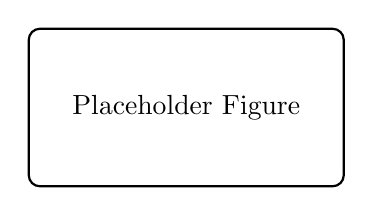
\begin{tikzpicture}
        \draw[thick, rounded corners] (0,0) rectangle (4,2) node[midway]{Placeholder Figure};
    \end{tikzpicture}
    \caption{Validation of the model under null conditions. This figure will be labeled as \textbf{Figure S1}.}
    \label{fig:supp_sim}
\end{figure}

\cref{fig:supp_sim} demonstrates the robustness of our $Z$-score calculation across different variance scales.
        \begin{singlespace}
            \printbibliography[title={References for Supplementary Notes}]
        \end{singlespace}
    \end{refsection}

\end{document}